%-------------------------------------------------------------------------------
\section{Background}
\label{sec:background}
%-------------------------------------------------------------------------------

In this section, we provide additional context on some concepts that we refer to
throughout the text.

\paragraph{Performance-enhancing proxies.}

The idea of in-network assistance has long brought pain to the hearts of
Internet researchers, protocol designers, and network operators. In particular,
the word ``middleboxes'' is often associated with NATs, firewalls, and other
policy enforcers that modify or inspect data in ways that break end-to-end
behavior. A substantial percentage of Internet paths are affected by feature or
protocol-breaking policies of middleboxes~\cite{edeline2019bottomup}.

In contrast, we refer specifically to the type of assistance provided by
performance-enhancing ``proxies'', or PEPs, that transparently split a TCP
connection in two~\cite{rfc3135}. While PEPs still interfere with end-to-end
transport mechanisms, their goal is to enhance the user experience by
maximizing performance, as opposed to enforce security or routing policies.

% \thea{Somewhere here, discuss the performance metrics PEPs can impact and then
%  limit our paper to the metrics we are interested in.}
Connection-splitting PEPs can enhance performance in several ways. By providing
an intermediate point of acknowledgment and retransmission, PEPs reduce the
length of the feedback loop for signals of loss and congestion. The PEP also
allows each side of the split connection to better optimize congestion control
and flow control for network conditions local to the path segment. We can
expect PEPs to impact a variety of performance metrics, including startup time,
packet jitter, retransmission overheads, and more. In this paper, we focus
only on the impact of connection-splitting on the \textit{sustained throughput}
of long-lived data transfers.

\paragraph{Congestion control.}

Congestion control was originally deployed in the 1980s to manage the explosive
growth of the Internet~\cite{vjk}. Foundational algorithms such as slow start
and fast retransmit eventually became part of the Tahoe congestion control
scheme. Variants such as NewReno and CUBIC emerged over time to improve
performance with fairness~\cite{ha2008cubic}. CUBIC is the default congestion control module for
TCP in the Linux kernel, and widely deployed. It is the primary ``loss-based''
congestion control scheme that we evaluate.

The word ``TCP'' is sometimes used synonomously with the congestion control
algorithms that it implements. In reality, the two are distinct, though deeply
intertwined. For example, the QUIC transport protocol implements many of the
same algorithms as TCP to manage network traffic, even though it runs over UDP~\cite{rfc9000}.
In this paper, we refer to ``TCP'' and ``QUIC'' as the transport protocols,
``Linux TCP'' as the implementation of TCP in the Linux kernel, and congestion
control schemes as the particular manifestations of a congestion control
algorithm in a transport protocol implementation.

\paragraph{BBR.}

Today, the focus on congestion control has shifted towards BBR. BBR is sometimes
referred to as a ``model-based'' congestion control scheme because it relies on
a fundamentally different approach of modeling network bandwidth and round-trip
time. It does not use packet loss as the primary signal for congestion. Google
initially presented BBR in 2016 as addressing the problems of CUBIC in
high-speed networks~\cite{cardwell2016bbr-ietf97}.

Over time, BBR encountered controversy for its unfairness towards loss-based
schemes~\cite{ware2019modeling,philip2021revisiting,cao2019use}. In response,
``v1'' of BBR has now evolved into BBRv2 in 2019 and BBRv3 in 2023, driven by
efforts at Google. Today, Google recommends that BBRv1 and BBRv2 be
deprecated in favor of BBRv3~\cite{cardwell2024bbrv3-ietf119}.

BBR is also widely deployed~\cite
{cardwell2024bbrv3-ietf119-qna,ware2024ccanalyzer}. Google has contributed BBR
implementations to the Linux kernel, and Amazon, Akamai, Meta, and Cloudflare
CDNs all use BBRv1 for TCP. At Google, BBRv3 is used in all google.com and
YouTube public Internet traffic with TCP, and is currently being A/B tested
against BBRv1 in Google QUIC traffic~\cite{cardwell2024bbrv3-ietf119}.
It is estimated that 40\% of traffic used BBR in 2019~\cite{mishra2019great}.

% https://datatracker.ietf.org/doc/draft-cardwell-ccwg-bbr/history/
Since 2017, there have been ongoing efforts to standardize BBR in the IETF~\cite{cardwell2024bbr-ietf-draft}.
However, progress has been slow. The Internet draft goes years or months at a
time without an update at the mercy of Google contributors. While companies
have been quick to adopt BBR in Linux TCP, adoption in QUIC has been slower.
Anecdotally, some have resorted to reverse engineering the Linux
implementation, and some such as Cloudflare, Meta, and Cisco are actively
experimenting with variants of BBRv2+ in their QUIC stacks~\cite
{cardwell2024bbrv3-ietf119-qna}.

% \begin{figure}
    \centering
    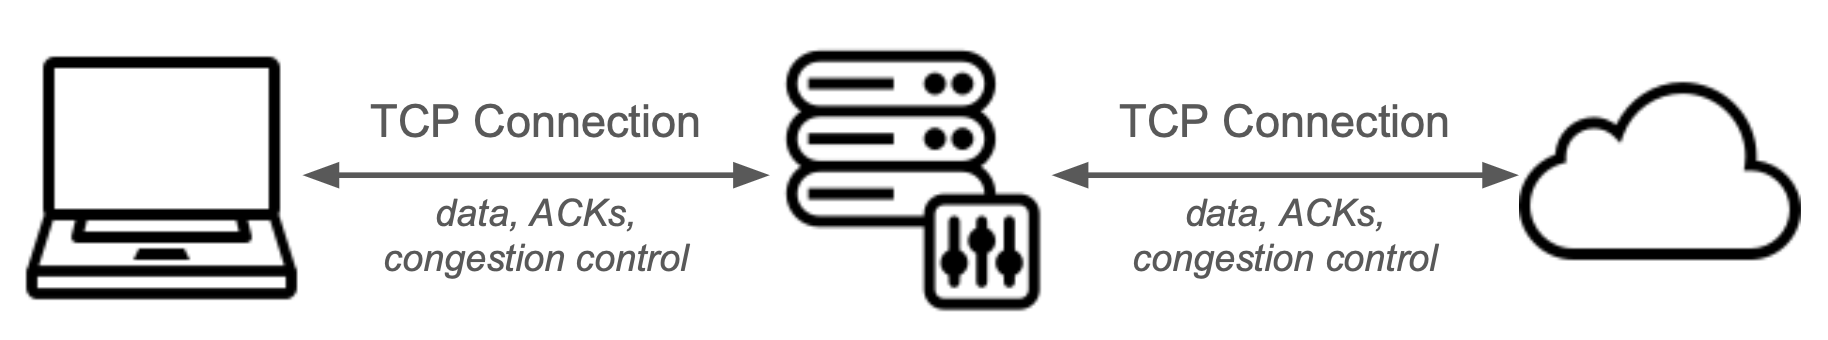
\includegraphics[width=\linewidth]{figures/pep_img_example.jpg}
    \caption{Diagram of a connection-splitting TCP PEP.}
    \label{fig:pep}
\end{figure}


\paragraph{QUIC.}

The QUIC transport protocol was originally developed by Google in 2012 to
improve performance for HTTPS traffic and to enable the rapid
evolution of transport mechanisms. QUIC is implemented over UDP, and moves
congestion control development from kernel space to user space.

As of 2021, QUIC is now a standards-track RFC~\cite{rfc9000} with widespread
deployment and interoperability testing~\cite{quic-interop}. It is estimated
that 8.4\% of global websites support QUIC~\cite{w3techs}, many of them major
traffic sources such as Cloudflare.
Still, many high-speed flows remain on TCP due to better TCP hardware
capabilities and ``per-origin'' caching, which complicates multi-CDN
deployments that mix protocols.
% Major traffic sources (e.g., Meta, Cloudflare, Google) make up a
% disproportionate share of traffic and support QUIC, but many high-speed flows
% are still over TCP because of superior TCP hardware offload capability in NICs,
% or because QUIC caching is done on a ``per-origin'' basis, meaning it's not
% possible to have a multi-CDN deployment where one CDN supports QUIC and another
% doesn't.

Evaluations of QUIC at the Internet scale generally show improved performance
compared to TCP, except in satellite networks. Features like zero-RTT
connection establishment and stream multiplexing enable measured improvements
in search latency, rebuffer rate, and other video playback metrics at
Google~\cite{langley2017quic}. Satellite network operators, on the other hand,
experience strife when it comes to QUIC. Several studies have measured the
negative impact of encryption on performance in split satellite
environments~\cite
{kosek2022quicpep,martin2022suitability,kuhn2021quic-over-sat,border2022evaluating}.
